\documentclass[11pt]{article}
\usepackage[margin=1in]{geometry}
\usepackage{amsmath, amssymb, amsthm}
\usepackage{booktabs}
\usepackage{hyperref}
\usepackage{xcolor}
% \usepackage{algorithm}    % not used in this document
% \usepackage{algpseudocode} % not used in this document
\usepackage{bm}
\usepackage{tikz}
\usetikzlibrary{positioning, calc, arrows.meta, decorations.pathreplacing}

\definecolor{emphasis}{HTML}{4A90D9}
\definecolor{warning}{HTML}{D95B5B}

\newcommand{\R}{\mathbb{R}}
\newcommand{\vect}[1]{\bm{#1}}
\newcommand{\mat}[1]{\mathbf{#1}}
\newcommand{\T}{\mathsf{T}}

\title{\textbf{Spectral Probing of the GigaPath Backbone}\\[4pt]
\large Jacobian Singular Value Analysis as a Dynamical Systems Diagnostic}
\author{autopath}
\date{}

\begin{document}
\maketitle
\thispagestyle{empty}

%% ================================================================
\section{Motivation: Layers as a Dynamical System}

We regard the depth-wise application of transformer blocks in the GigaPath
backbone as a discrete-time dynamical system.  Let $\vect{h}_l \in \R^{N
\times d}$ denote the token-sequence hidden state at layer~$l$, where $N$
is the number of tokens (including the CLS token) and $d = 1536$ is the
embedding dimension.  Each transformer block defines the recurrence
\begin{equation}\label{eq:dynamics}
    \vect{h}_{l+1} = F_l(\vect{h}_l;\, \theta_l)
        = \vect{h}_l + G_l(\vect{h}_l;\, \theta_l),
\end{equation}
where $G_l$ is the residual branch (self-attention $\to$ layer-scale
$\to$ MLP $\to$ layer-scale) and $\theta_l$ collects the parameters of
block~$l$.  The total depth is $L = 40$.

\paragraph{Attractor hypothesis.}
After self-supervised pre-training the system~\eqref{eq:dynamics} has
converged to a regime in which input representations are mapped to a
low-dimensional attractor.  The geometry of this attractor is
characterised by the \emph{Lyapunov spectrum}: the rates at which
infinitesimally nearby trajectories (i.e.\ nearby inputs) diverge or
converge as they propagate through the layers.

%% ================================================================
\section{GigaPath Backbone Architecture}

The GigaPath tile encoder is a DINOv2-giant Vision Transformer (ViT-g)
with $L=40$ layers, embedding dimension $d=1536$, $24$ attention heads
(head dimension $d_h=64$), and a SwiGLU MLP with hidden dimension $4096$
(gated via an $8192$-wide intermediate).  The full architecture is shown
in Figure~\ref{fig:backbone}.

\begin{figure}[htp]
\centering
\resizebox{\textwidth}{!}{%
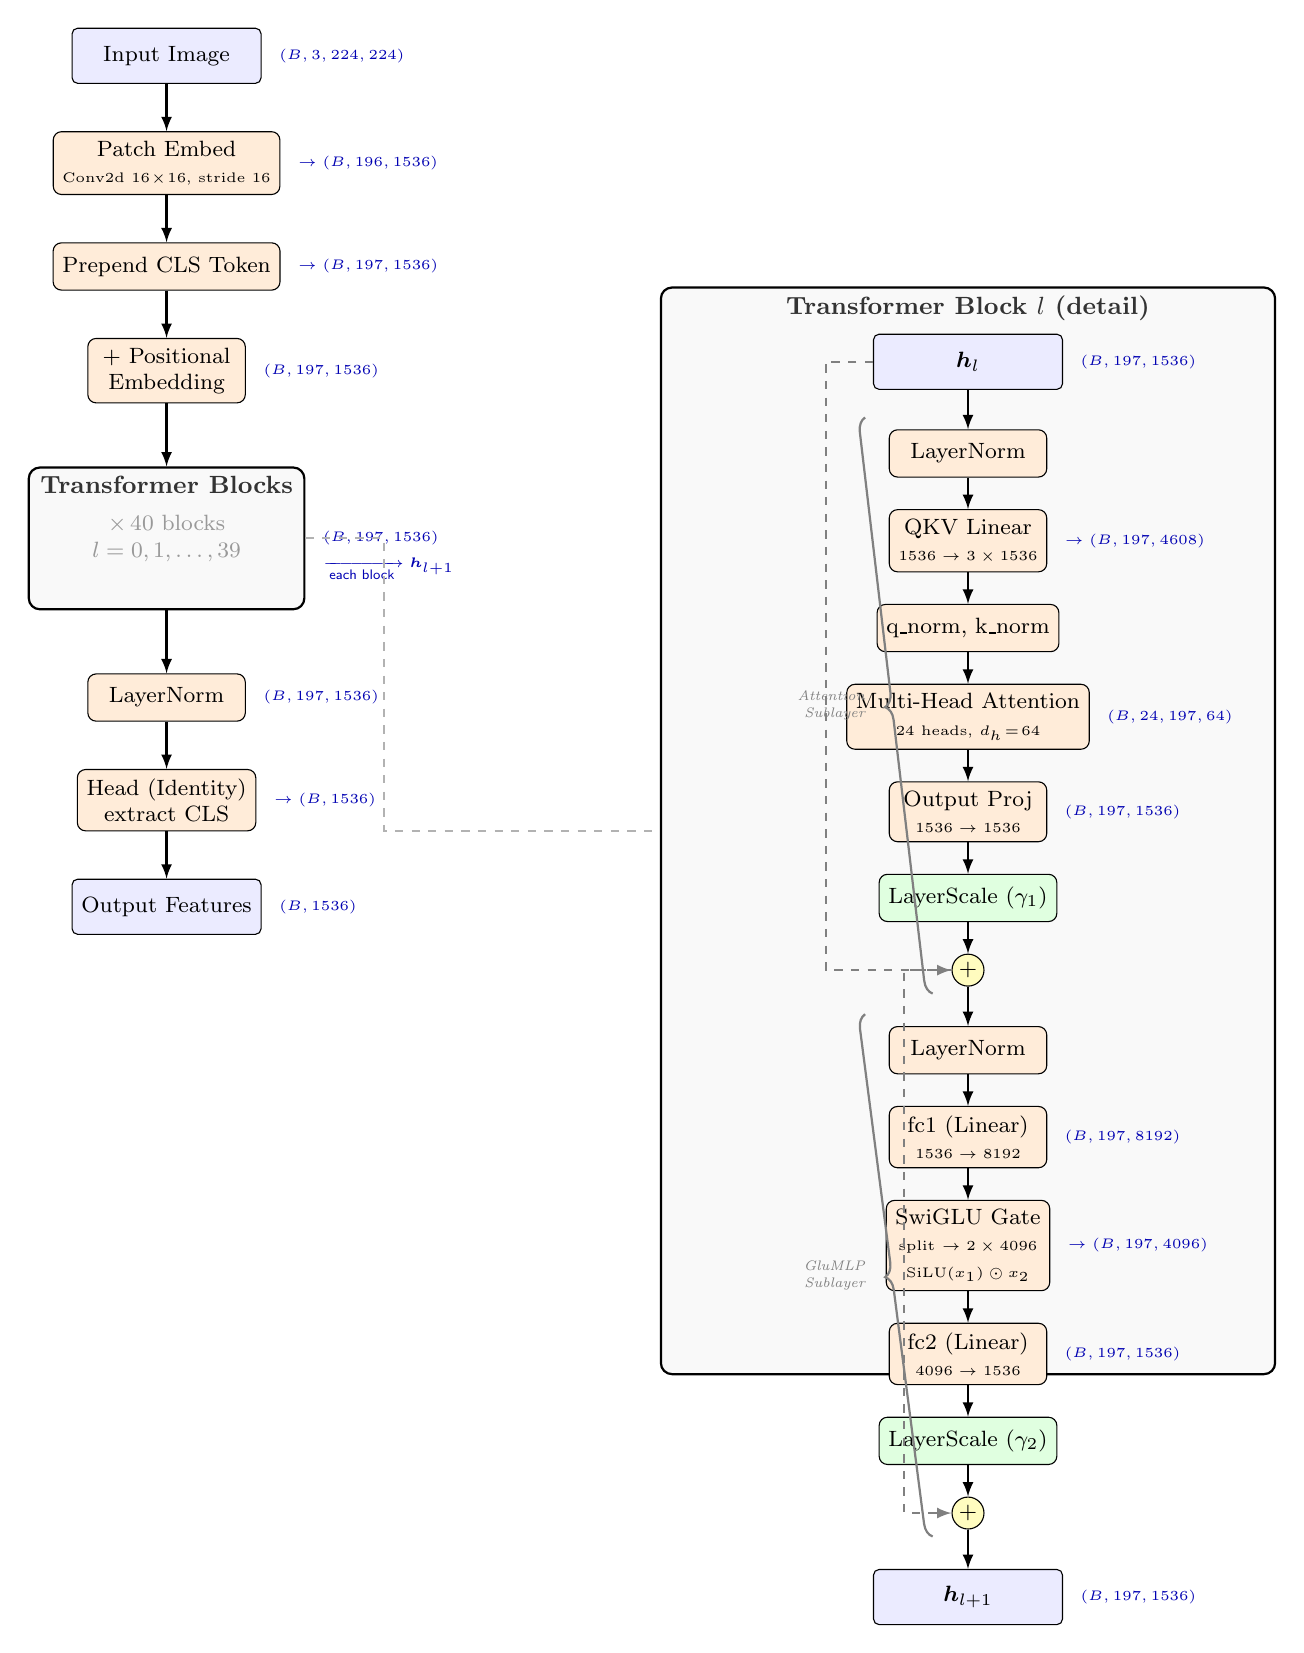
\begin{tikzpicture}[
    >=latex,
    node distance=0.9cm and 1.4cm,
    % Styles
    tensor/.style={draw, rounded corners=2pt, fill=blue!8,
        minimum height=0.7cm, minimum width=2.4cm, font=\footnotesize,
        align=center},
    op/.style={draw, rounded corners=3pt, fill=orange!15,
        minimum height=0.6cm, minimum width=2.0cm, font=\footnotesize,
        align=center},
    branch/.style={draw, rounded corners=3pt, fill=green!12,
        minimum height=0.6cm, minimum width=2.0cm, font=\footnotesize,
        align=center},
    residual/.style={draw, circle, fill=yellow!25, inner sep=1pt,
        font=\footnotesize},
    dim/.style={font=\tiny\sffamily, text=blue!70!black},
    arr/.style={->, thick},
    darr/.style={->, thick, dashed, gray},
    block/.style={draw, thick, rounded corners=4pt, fill=gray!5,
        inner sep=6pt},
    blockhead/.style={font=\small\bfseries, text=black!80},
]

% ===== Left column: full pipeline =====
\node[tensor] (img) {Input Image};
\node[dim, right=0.1cm of img] {$(B,3,224,224)$};

\node[op, below=0.6cm of img] (patch) {Patch Embed\\{\tiny Conv2d $16\!\times\!16$, stride $16$}};
\draw[arr] (img) -- (patch);
\node[dim, right=0.1cm of patch] {$\to (B,196,1536)$};

\node[op, below=0.6cm of patch] (cls) {Prepend CLS Token};
\draw[arr] (patch) -- (cls);
\node[dim, right=0.1cm of cls] {$\to (B,197,1536)$};

\node[op, below=0.6cm of cls] (pos) {$+$ Positional\\Embedding};
\draw[arr] (cls) -- (pos);
\node[dim, right=0.1cm of pos] {$(B,197,1536)$};

% Transformer stack
\node[block, below=0.8cm of pos, minimum width=3.5cm, minimum height=1.8cm]
    (stack) {};
\node[blockhead, anchor=north] at (stack.north) {Transformer Blocks};
\node[font=\footnotesize, text=gray!80, align=center] at (stack.center)
    {$\times\, 40$ blocks\\$l = 0, 1, \ldots, 39$};
\draw[arr] (pos) -- (stack.north);
\node[dim, right=0.1cm of stack] {$(B,197,1536)$};
\node[dim, right=0.1cm of stack, yshift=-0.4cm]
    {$\xrightarrow[\text{each block}]{} \vect{h}_{l+1}$};

\node[op, below=0.8cm of stack] (norm) {LayerNorm};
\draw[arr] (stack.south) -- (norm);
\node[dim, right=0.1cm of norm] {$(B,197,1536)$};

\node[op, below=0.6cm of norm] (head) {Head (Identity)\\extract CLS};
\draw[arr] (norm) -- (head);
\node[dim, right=0.1cm of head] {$\to (B,1536)$};

\node[tensor, below=0.6cm of head] (out) {Output Features};
\draw[arr] (head) -- (out);
\node[dim, right=0.1cm of out] {$(B,1536)$};

% ===== Right column: single block detail =====
% Position the detail block to the right
\coordinate (detailorigin) at ($(stack.east) + (4.5cm, 3.2cm)$);

\node[block, anchor=north west, minimum width=7.8cm, minimum height=13.8cm]
    (detail) at (detailorigin) {};
\node[blockhead, anchor=north] at (detail.north)
    {Transformer Block $l$ (detail)};

% --- Input ---
\node[tensor, below=0.6cm of detail.north] (hin)
    {$\vect{h}_l$};
\node[dim, right=0.1cm of hin] {$(B,197,1536)$};

% --- Attention Sublayer ---
\node[op, below=0.5cm of hin] (ln1) {LayerNorm};
\draw[arr] (hin) -- (ln1);

\node[op, below=0.4cm of ln1] (qkv)
    {QKV Linear\\{\tiny $1536 \to 3 \times 1536$}};
\draw[arr] (ln1) -- (qkv);
\node[dim, right=0.1cm of qkv] {$\to (B,197,4608)$};

\node[op, below=0.4cm of qkv] (qknorm)
    {q\_norm, k\_norm};
\draw[arr] (qkv) -- (qknorm);

\node[op, below=0.4cm of qknorm] (mha)
    {Multi-Head Attention\\{\tiny 24 heads, $d_h\!=\!64$}};
\draw[arr] (qknorm) -- (mha);
\node[dim, right=0.1cm of mha] {$(B,24,197,64)$};

\node[op, below=0.4cm of mha] (proj)
    {Output Proj\\{\tiny $1536 \to 1536$}};
\draw[arr] (mha) -- (proj);
\node[dim, right=0.1cm of proj] {$(B,197,1536)$};

\node[branch, below=0.4cm of proj] (ls1)
    {LayerScale ($\gamma_1$)};
\draw[arr] (proj) -- (ls1);

% Residual Add 1
\node[residual, below=0.4cm of ls1] (add1) {$+$};
\draw[arr] (ls1) -- (add1);
% Residual skip from input
\draw[darr] (hin.west) -- ++(-0.6cm,0) |- (add1.west);

% --- MLP Sublayer ---
\node[op, below=0.5cm of add1] (ln2) {LayerNorm};
\draw[arr] (add1) -- (ln2);

\node[op, below=0.4cm of ln2] (fc1)
    {fc1 (Linear)\\{\tiny $1536 \to 8192$}};
\draw[arr] (ln2) -- (fc1);
\node[dim, right=0.1cm of fc1] {$(B,197,8192)$};

\node[op, below=0.4cm of fc1] (gate)
    {SwiGLU Gate\\{\tiny split $\to 2 \times 4096$}\\
     {\tiny SiLU$(x_1) \odot x_2$}};
\draw[arr] (fc1) -- (gate);
\node[dim, right=0.1cm of gate] {$\to (B,197,4096)$};

\node[op, below=0.4cm of gate] (fc2)
    {fc2 (Linear)\\{\tiny $4096 \to 1536$}};
\draw[arr] (gate) -- (fc2);
\node[dim, right=0.1cm of fc2] {$(B,197,1536)$};

\node[branch, below=0.4cm of fc2] (ls2)
    {LayerScale ($\gamma_2$)};
\draw[arr] (fc2) -- (ls2);

% Residual Add 2
\node[residual, below=0.4cm of ls2] (add2) {$+$};
\draw[arr] (ls2) -- (add2);
% Residual skip from post-attention
\draw[darr] (add1.west) -- ++(-0.6cm,0) |- (add2.west);

% --- Output ---
\node[tensor, below=0.5cm of add2] (hout)
    {$\vect{h}_{l+1}$};
\draw[arr] (add2) -- (hout);
\node[dim, right=0.1cm of hout] {$(B,197,1536)$};

% --- Dashed line connecting main diagram to detail ---
\draw[thick, dashed, gray!60]
    (stack.east) -- ++(1.0cm,0) |- (detail.west);

% --- Braces for sublayer labels ---
\draw[decorate, decoration={brace, amplitude=5pt, mirror}, thick, gray]
    ($(ln1.north west) + (-0.3cm, 0.15cm)$) --
    ($(add1.south west) + (-0.3cm, -0.15cm)$)
    node[midway, left=0.3cm, font=\tiny\itshape, text=gray, align=right]
    {Attention\\Sublayer};

\draw[decorate, decoration={brace, amplitude=5pt, mirror}, thick, gray]
    ($(ln2.north west) + (-0.3cm, 0.15cm)$) --
    ($(add2.south west) + (-0.3cm, -0.15cm)$)
    node[midway, left=0.3cm, font=\tiny\itshape, text=gray, align=right]
    {GluMLP\\Sublayer};

\end{tikzpicture}%
}
\caption{Architecture of the GigaPath tile backbone
    (DINOv2-giant ViT-g/14, $L=40$, $d=1536$, $24$ heads).
    \textbf{Left}: full forward pipeline from input image to output
    feature vector.
    \textbf{Right}: expanded view of a single transformer block~$l$,
    showing the attention sublayer with $\text{QKV} \to \text{MHSA}
    \to \text{Proj} \to \text{LayerScale} \to \text{Residual}$, and the
    GluMLP sublayer with $\text{fc1} \to \text{SwiGLU} \to \text{fc2}
    \to \text{LayerScale} \to \text{Residual}$.
    Dashed arrows indicate residual skip connections.
    All tensor shapes are annotated in
    {\color{blue!70!black}\textsf{blue}}.}
\label{fig:backbone}
\end{figure}

%% ================================================================
\section{Which Jacobian?}

Two natural Jacobians can be defined at every layer:

\begin{center}
\begin{tabular}{lll}
\toprule
\textbf{Symbol} & \textbf{Definition} & \textbf{Measures} \\
\midrule
$\mat{J}_l^{(h)} = \dfrac{\partial \vect{h}_{l+1}}{\partial \vect{h}_l}$ &
    State-space Jacobian &
    Sensitivity of output to \emph{hidden state} perturbations \\[8pt]
$\mat{J}_l^{(\theta)} = \dfrac{\partial \vect{h}_{l+1}}{\partial \theta_l}$ &
    Parameter Jacobian &
    Sensitivity of output to \emph{weight} perturbations \\
\bottomrule
\end{tabular}
\end{center}

\paragraph{For Lyapunov analysis, use the state-space Jacobian $\mat{J}_l^{(h)}$.}
Lyapunov exponents characterise how nearby \emph{trajectories} (hidden
states produced by nearby inputs) diverge or converge.  This is entirely
governed by $\mat{J}_l^{(h)}$.  The parameter Jacobian
$\mat{J}_l^{(\theta)}$ measures Fisher-information-type sensitivities,
which is a different (though related) diagnostic.

The residual structure~\eqref{eq:dynamics} implies
\begin{equation}\label{eq:jacobian-residual}
    \mat{J}_l^{(h)}
        = \mat{I} + \frac{\partial G_l}{\partial \vect{h}_l},
\end{equation}
so the Jacobian is a perturbation of the identity.

%% ================================================================
\section{Singular Values and the Lyapunov Spectrum}

\subsection{Notation}

Let $\sigma_i^{(l)}$ denote the $i$-th singular value of
$\mat{J}_l^{(h)}$, i.e.\
\begin{equation}
    \sigma_i^{(l)} \;=\; \sigma_i\!\bigl(\mat{J}_l^{(h)}\bigr)
        \;=\; \sqrt{\lambda_i\!\bigl(\mat{J}_l^{(h)\T}\, \mat{J}_l^{(h)}\bigr)},
\end{equation}
where $\lambda_i(\cdot)$ denotes the $i$-th eigenvalue (in decreasing
order).  In other words, $\sigma_i^{(l)}$ is the $i$-th singular value
of the layer-$l$ Jacobian, measuring the local expansion ($\sigma > 1$)
or contraction ($\sigma < 1$) rate in the $i$-th principal direction at
that layer.

\begin{itemize}
    \item $\sigma_i^{(l)} > 1$: the $i$-th direction is \textbf{expanded} by layer~$l$ --- information is amplified.
    \item $\sigma_i^{(l)} < 1$: the $i$-th direction is \textbf{contracted} --- information is discarded.
    \item $\sigma_i^{(l)} \approx 1$: the $i$-th direction is approximately \textbf{preserved} (dynamical isometry).
\end{itemize}

\subsection{Finite-depth Lyapunov exponents}

The (finite-depth) Lyapunov exponents of the system are defined by the
singular values of the composed mapping $\mat{J}^{[0:L]} = \prod_{l=0}^{L-1} \mat{J}_l^{(h)}$.
Concretely, by the multiplicative ergodic theorem (Oseledets, 1968), the
Lyapunov exponents are
\begin{equation}\label{eq:lyapunov}
    \Lambda_i
        \;=\; \lim_{L\to\infty}\;
              \frac{1}{2L}\,
              \log \lambda_i\!
              \Bigl(\prod_{l=0}^{L-1} \mat{J}_l^{(h)\T}\, \mat{J}_l^{(h)}\Bigr).
\end{equation}
For a finite-depth network, we replace the limit with a finite sum and
define the \emph{empirical Lyapunov exponents} as
\begin{equation}\label{eq:emp-lyapunov}
    \hat\Lambda_i
        \;=\; \frac{1}{L} \sum_{l=0}^{L-1} \log \sigma_i^{(l)}.
\end{equation}
This is an approximation; strictly it assumes the singular-value
directions align across layers, but it provides a useful summary
statistic.

\paragraph{Key observables.}
\begin{center}
\begin{tabular}{ll}
\toprule
\textbf{Observable} & \textbf{Interpretation} \\
\midrule
$\sigma_{\max}^{(l)} \gg 1$
    & Layer~$l$ strongly amplifies certain directions \\
$\sigma_{\min}^{(l)} \ll 1$
    & Layer~$l$ strongly contracts certain directions \\
$\kappa^{(l)} = \sigma_{\max}^{(l)} / \sigma_{\min}^{(l)} \gg 1$
    & High condition number; anisotropic geometry \\
All $\sigma_i^{(l)} \approx 1$
    & Dynamical isometry (ideal for signal propagation) \\
$\hat\Lambda_i > 0$
    & Net expansion over the full depth --- chaos-like regime \\
$\hat\Lambda_i < 0$
    & Net contraction --- attractor-like regime \\
$\hat\Lambda_i \approx 0$
    & Critical regime (edge of chaos) \\
\bottomrule
\end{tabular}
\end{center}

\subsection{Why the residual structure matters}
From~\eqref{eq:jacobian-residual}, $\mat{J}_l^{(h)} = \mat{I} +
\partial G_l/\partial \vect{h}_l$, so
$\sigma_i^{(l)} = 1 + \delta_i^{(l)}$ where $\delta_i^{(l)}$ are the
singular-value perturbations introduced by the residual branch.
The interesting diagnostic is the \emph{deviation spectrum}
$\{\delta_i^{(l)}\}$, or equivalently $\{\log\sigma_i^{(l)}\}$,
plotted as a function of layer index~$l$.

\subsection{Input dependence}
Because transformers use attention, $\mat{J}_l^{(h)}$ depends on the
input $\vect{h}_l$, which itself depends on the data point.  The spectral
probe therefore produces a \emph{per-sample} local Lyapunov spectrum.  In
practice, we aggregate by averaging singular values (or their logs) over
a mini-batch.

%% ================================================================
\section{Feasibility of the Attractor Hypothesis}

The hypothesis is well-supported by prior work:

\begin{enumerate}
    \item \textbf{Deep Information Propagation} (Schoenholz et~al., 2017):
        at initialisation, deep networks must operate at the edge of chaos
        (all Lyapunov exponents $\approx 0$) for trainability.

    \item \textbf{Dynamical isometry} (Saxe et~al., 2014; Pennington
        et~al., 2018): well-trained networks have Jacobian singular values
        clustered near~$1$.

    \item \textbf{Residual networks} (Yang \& Schoenholz, 2018): residual
        connections bias $\mat{J}$ toward the identity, naturally
        promoting dynamical isometry.

    \item \textbf{For a frozen pre-trained ViT} such as GigaPath, the
        expectation is that most $\sigma_i^{(l)} \approx 1$, with a few
        extreme values encoding the dominant feature-transformation modes.
        The largest singular values correspond to the directions the
        network \emph{amplifies} (semantically important features), and
        the smallest to the directions it \emph{discards}.
\end{enumerate}


%% ================================================================
\section{Efficient Computation}

\subsection{Dimensionality}

With $N = 197$ tokens (196 patches + CLS) and $d = 1536$, the full
Jacobian $\mat{J}_l^{(h)} \in \R^{Nd \times Nd}$ has dimension
$302{,}592 \times 302{,}592$.  Materialising or decomposing this matrix
is infeasible.

\subsection{Two modes of operation}

We implement two complementary modes:

\paragraph{Mode~1: CLS-token-only (materialisable).}
If we restrict to the CLS token (the first row of the token sequence),
the Jacobian reduces to
\begin{equation}
    \mat{J}_l^{\text{cls}} \;=\;
        \frac{\partial [\vect{h}_{l+1}]_{\text{cls}}}
             {\partial [\vect{h}_l]_{\text{cls}}}
    \;\in\; \R^{d \times d},
\end{equation}
where $d = 1536$.  This $1536 \times 1536$ matrix can be materialised
directly via \texttt{torch.autograd.functional.jacobian} and decomposed
with standard dense SVD in $\sim\!1$ second on GPU.  This gives a
complete spectrum of all 1536 singular values.

\paragraph{Mode~2: Full-sequence matrix-free (via JVP/VJP).}
For the full $Nd \times Nd$ Jacobian, we avoid materialisation entirely.
We define a \texttt{scipy.sparse.linalg.LinearOperator} that implements
the matrix-vector products
\begin{align}
    \text{matvec:}  & \quad \vect{u} = \mat{J}\,\vect{v}
        \quad\text{via}\quad \texttt{torch.func.jvp}
        \label{eq:jvp}\\
    \text{rmatvec:} & \quad \vect{v} = \mat{J}^\T\!\vect{u}
        \quad\text{via}\quad \texttt{torch.func.vjp}
        \label{eq:vjp}
\end{align}
and then call \texttt{scipy.sparse.linalg.svds} to obtain the top-$k$
and bottom-$k$ singular values via implicitly-restarted Lanczos
bidiagonalisation.  Each call to~\eqref{eq:jvp} or~\eqref{eq:vjp} has
the cost of one forward or backward pass through a \emph{single}
transformer block.

\subsection{Overall cost}

\begin{center}
\begin{tabular}{lcc}
\toprule
\textbf{Mode} & \textbf{Cost per layer} & \textbf{Output} \\
\midrule
CLS-only &
    $\sim\!d^2$ forward ops $+$ dense SVD &
    All $d$ singular values \\
Matrix-free, top/bottom $k$ &
    $\sim\!(2k \cdot n_{\text{iter}})$ block fwd/bwd passes &
    Top-$k$ and bottom-$k$ singular values \\
\bottomrule
\end{tabular}
\end{center}

Probing 5 evenly-spaced blocks with $k=10$ in matrix-free mode requires
$\sim\!5\times 2\times 10\times 20 = 2000$ block evaluations (assuming
$n_{\text{iter}}\approx 20$ Lanczos steps), versus 40 blocks for one
full forward pass.  This is $\sim\!50\times$ overhead \emph{per probed
sample}, so the probe should be run on a small batch (e.g.\ 1--4
samples) and not on every evaluation step.  The CLS-only mode is far
cheaper ($\sim\!3$--$5\times$ one forward pass for 5 blocks) and is
recommended for routine monitoring.


%% ================================================================
\section{Implementation}

\subsection{\texttt{SpectralProbe}: standalone spectral estimator}

Given a transformer block $F_l$ and an activation tensor
$\vect{h}_l$, the \texttt{SpectralProbe} estimates:

\begin{itemize}
    \item \textbf{CLS mode}: materialises
        $\mat{J}_l^{\text{cls}} \in \R^{d\times d}$ via
        \texttt{torch.autograd.functional.jacobian}, then calls
        \texttt{torch.linalg.svdvals}.
    \item \textbf{Full mode}: wraps JVP/VJP in a
        \texttt{LinearOperator} and calls
        \texttt{scipy.sparse.linalg.svds} for top/bottom~$k$.
\end{itemize}

\subsection{\texttt{SpectralBackboneEvaluator}: integrated evaluator}

\texttt{SpectralBackboneEvaluator} subclasses
\texttt{SidebandBackboneEvaluator}.  It reuses the existing hook
infrastructure to capture intermediate activations at the probed blocks,
then runs \texttt{SpectralProbe} on those activations after the forward
pass.  Results are stored in the \texttt{spectral\_results} property,
keyed by block index.

The evaluator is instantiated via \texttt{gigapath\_backbone\_evaluator}
with name \texttt{"GIGAPATH\_SPECTRAL\_BACKBONE\_5BLOCK\_EVALUATOR"}.


\subsection{Pipeline entry point}

In \texttt{pipelines.py}:

\begin{verbatim}
gigapath_backbone_evaluator(
    "GIGAPATH_BASELINE_BACKBONE_SPECTRAL_EVALUATOR",
    device='cuda',
)
\end{verbatim}

This returns a \texttt{SpectralBackboneEvaluator} that probes 5
evenly-spaced blocks (indices 0, 10, 20, 30, 39) and estimates both the
CLS-only full spectrum and the top/bottom 10 matrix-free singular values.


%% ================================================================
\section{Interpretation Guide}

Plot $\log\sigma_i^{(l)}$ versus layer index~$l$ for the top and bottom
singular values.  Expected patterns for a well-trained ViT:

\begin{enumerate}
    \item \textbf{Most singular values near~1} (i.e.\
        $\log\sigma \approx 0$): the network is approximately isometric,
        preserving the geometry of the representation.

    \item \textbf{A few large singular values} ($\sigma \gg 1$):
        these correspond to directions the network selectively amplifies
        --- likely the most semantically discriminative feature
        directions.

    \item \textbf{A few small singular values} ($\sigma \ll 1$):
        these correspond to directions being aggressively compressed ---
        the network is performing dimensionality reduction along these
        directions.

    \item \textbf{Singular values converging as $l$ increases}: this
        supports the attractor hypothesis --- later layers are ``closer''
        to the fixed point, with the Jacobian becoming more isometric.

    \item \textbf{Condition number $\kappa^{(l)}$ decreasing with depth}:
        further evidence of convergence to an attractor with decreasing
        anisotropy.
\end{enumerate}


\end{document}
